\chapter{Performance Evaluation}

\section{Theoretical Performance}

In this section, we analyze the performance of \Sys, and compare the performance of our work with other prior schemes. Our analysis ignores the relatively trivial cost like Fast Fourier Transform (FFT) and focuses on the heavy work such as multi-scalar multiplication (MSM) and group operations. Our analysis also ignores the differences of the implementations and assumes each protocol is executed in a single thread.
\subsection{Proof of Assets}

We use $\kappa$ to denote the size of the anonymity set and we assume $\kappa$ is the power of two for simplicity. The performance analysis of \bootstrap and \userproof are performed as follows:
\begin{itemize}
\item \bootstrap: For each public key in the anonymity set, $\prv$ opens an evaluation of the KZG commitment and generates the corresponding proof of the $\Sigma$-protocol in Protocol~\ref{alg:boot}. When opening an evaluation of a KZG commitment, one MSM for the witness and one MSM for the blinding polynomial are involved. The number of scalar multiplications of the $\Sigma$-protocol is constant. Thus, the overhead proving time of \bootstrap is $O(\kappa^2)$. In terms of verifier's work, $\vrf$ does not need to perform MSM to verify the proofs; $\vrf$ computes scalar multiplications for constant times instead. To verify the committed values are correct, $\vrf$ manipulates the batched KZG scheme rather than verifying each proof one by one, which means $O(1)$ verifying time and proof size for each public key. Therefore, the overhead verifying time and proof size of \bootstrap is $O(\kappa)$.
\item \poa: $\prv$ constructs the accumulator and commits to constant number of polynomials. According to Schwartz-Zippel lemma, $\prv$ only needs to open one point of each polynomial. Thus, the proving time is $O(\kappa)$ and the proof size is $O(1)$ because the number of polynomial commitments is constant. While it takes constant time for $\vrf$ to verify the proof of the PCS, $\vrf$ needs to process the inputs, \ie interpolates the balances and commits to the balance polynomial, which means one MSM involved. Therefore, the overhead verifier's work of \poa is $O(\kappa)$.
\end{itemize}

\subsection{Proof of Liability}
We use $\mu$ to denote the number of users and $k$ to denote the allowed size of the range proof. Recall that $\prv$ needs to construct several polynomials for the range proof. Although the number of the range-proof polynomials is arbitrary, $2^{64}$ is sufficient for almost all the exchanges' requirements in the real world, which means there are less than or equal to 64 polynomials for the range proof. Therefore, we can treat the number of range-proof polynomials as a constant, but we still use $k$ to indicate the performance is related to the range proof. $\prv$ also needs to compute the accumulative polynomial to prove the total liability is correct, which can be done in linear time. Different from \bootstrap, $\prv$ only opens each polynomial at one random evaluation point. Thus, the proving time is $O(\mu)$.
The verifier's work is broken into \userproof and \pol:
\begin{itemize}
\item \userproof: Each user verifies his balance is the evaluation of the polynomial $p_1$ and his user identifier is the evaluation of the polynomial $f_\mathsf{uid}$, and the two evaluation points should be the same. The user checks two proofs of KZG commitment, so the proof size and the verifying time for customers are both $O(1)$.
\item \pol: Auditor verifies the constraints among polynomials $\{p_i\}$ are correct and the committed total liability is the evaluation of $f_\mathsf{liab}(\omega^0)$. The verification of constraints requires two steps: 1. validating each opening evaluation is correct; 2. the evaluations of $\{w_1,w_2,v_1,v_2,\dots,v_k\}$ are zero. The first step can be done in constant time because the number of polynomials is related to the range proof rather than the number of users. The second step takes several scalar multiplications and group additions but still in constant times. Recall that the proof of KZG commitment consists of one witness, one evaluation, and the corresponding evaluation point, which are unrelated to the degree of the polynomial. That means the verifying time and the proof size for auditors are both $O(k)$.
\end{itemize}

\subsection{Comparison}

\begin{table*}[t]
\centering
\resizebox{\textwidth}{!}{
    \begin{tabular}{|c|c|c|c|c|c|c|c|} 
        \hline
        \multicolumn{7}{|c|}{$\pi_\mathsf{keys}$} \\
        \hline
        \textbf{Scheme} & \textbf{Proving time} & \textbf{Verifying time} & \textbf{Proof size} & \textbf{Hashed} & \textbf{NI} & \textbf{Incremental} \\
        \hline
        \Sys(\textbf{Ours}) & $O(\nkeys^2)$ & $O(\nkeys)$ & $O(\nkeys)$ & $\tikzcmark$ & $\tikzcmark$ & $\tikzxmark$ \\
        \hline
    \end{tabular}
}\\
\resizebox{\textwidth}{!}{
    \begin{tabular}{|c|c|c|c|c|c|c|c|} 
        \hline
        \multicolumn{8}{|c|}{$\pi_\mathsf{assets}$} \\
        \hline
        \multirow{2}{*}{\textbf{Scheme}} & \multirow{2}{*}{\textbf{Proving time}} & \multicolumn{2}{c|}{\textbf{Verifying time}} & \multirow{2}{*}{\textbf{Proof size}} & \multirow{2}{*}{\textbf{Hashed}} & \multirow{2}{*}{\textbf{NI}} & \multirow{2}{*}{\textbf{Incremental}} \\
        \cline{3-4}
        & & $\pi_\mathsf{input}$ & $\pi_\mathsf{proof}$ & & & & \\
        \hline
        Provisions\cite{provisions} & $O(\nkeys)$ & N/A & $O(\nkeys)$ & $O(\nkeys)$ & $\tikzxmark$ & $\tikzcmark$ & $\tikzxmark$ \\
        \hline
        Bulletproofs\cite{bulletproofs} & $O(\nkeys)$ & N/A & $O(\nkeys)$ & $O(\log{\nkeys})$ & $\tikzcmark$ & $\tikzcmark$ & $\tikzxmark$ \\
        \hline
        NIZKPCS\cite{composite} & $O(\nkeys\log\nkeys)$ & N/A & $O(\nkeys)$ & $O(\nkeys)$ & $\tikzcmark$ & $\tikzcmark$ & $\tikzxmark$ \\
        \hline
        gOTzilla\cite{gotzilla} & $O(\nkeys)$ & $O(\nkeys)$ & $O(\nkeys)$ & $O(\log{\nkeys})$ & $\tikzcmark$ & $\tikzxmark$ & $\tikzxmark$ \\
        \hline
        IZPR\cite{izpr} & $O(t\log{t})$ & $O(\nkeys)$ & $O(1)$ & $O(1)$ & $\tikzcmark$ & $\tikzcmark$ & $\tikzcmark$ \\
        \hline
        \Sys(\textbf{Ours}) & $O(\nkeys)$ & $O(\nkeys)$ & $O(1)$ & $O(1)$ & $\tikzcmark$ & $\tikzcmark$ & $\tikzxmark$ \\
        \hline
    \end{tabular}
}
    \caption[Comparison of this work with prior PoA schemes]{Comparison of this work with prior PoA schemes. $\pi_\mathsf{input}$ is the verifier processes the public inputs before validating the proof; $\pi_\mathsf{proof}$ is the verifier verifies the proof sent by the prover. \textbf{Hashed}: whether the scheme is compatible with hashed keys. \textbf{NI}: non-interactive. Notation: $\nkeys$ is the size of the anonymity set that the exchange wants to prove. For IZPR\cite{izpr}, $t$ is the throughput of the blockchain (number of addresses which have changed since the last proof).\label{tab:poa}}
\end{table*}

\begin{table*}[t]
\centering
\resizebox{\textwidth}{!}{
    \begin{tabular}{|c|c|c|c|c|c|c|} 
        \hline
        \multirow{2}{*}{\textbf{Scheme}} & \multirow{2}{*}{\textbf{Proving time}} & \multicolumn{2}{c|}{\textbf{Verifying time}} & \multicolumn{2}{c|}{\textbf{Proof size}} & \multirow{2}{*}{\textbf{Incremental}} \\
        \cline{3-6}
        & & $\pi_\mathsf{users}$ & $\pi_\mathsf{liabilities}$ & $\pi_\mathsf{users}$ & $\pi_\mathsf{liabilities}$ & \\
        \hline
        Provisions\cite{provisions} & $O(\nusers)$ & $O(1)$ & $O(\nusers)$ & $O(1)$ & $O(\nusers)$ & $\tikzxmark$ \\
        \hline
        DAPOL+\cite{dapol} & $O(\nusers\log{\nusers})$ & $O(\log{\nusers})$ & $O(1)$ & $O(\log{\nusers})$ & $O(1)$ & $\tikzxmark$ \\
        \hline
        SPPPOL\cite{spp} & $O(\log_{\lambda}{\nusers})$ & $O(\log_{\lambda}{\nusers})$ & $O(1)$ & $O(\log_{\lambda}{\nusers})$ & $O(1)$ & $\tikzxmark$ \\
        \hline
        Notus\cite{notus} & $O(\nusers\log{\nusers})$ & $O(1)$ & $O(1)$ & $O(1)$ & $O(1)$ & $\tikzcmark$ \\
        \hline
        \Sys(\textbf{Ours}) & $O(k\cdot{\nusers})$ & $O(1)$ & $O(k)$ & $O(1)$ & $O(k)$ & $\tikzxmark$ \\
        \hline
    \end{tabular}
}
    \caption[Comparison of this work with prior PoL schemes]{Comparison of this work with prior PoL schemes. Notation: $\nusers$ is the number of users, $k$ is the number of bits of the range proof. For SPPPOL \cite{spp}, $\lambda$ is the arity of the Verkle Tree it uses.\label{tab:pol}}
\end{table*}

In Table~\ref{tab:poa}, we compare this work with other prior PoA schemes. Both IZPR and this work utilize bootstrapping, but the bootstrapping of IZPR will be introduced in their following paper. We only analyze the performance of the bootstrapping for this work. In Table~\ref{tab:pol}, we compare this work with prior PoL schemes.

\section{Implementation and Benchmark Methodology}



\begin{figure*}[t]
    \begin{subfigure}{0.3\textwidth}
        \centering
        \resizebox{\linewidth}{!}{
            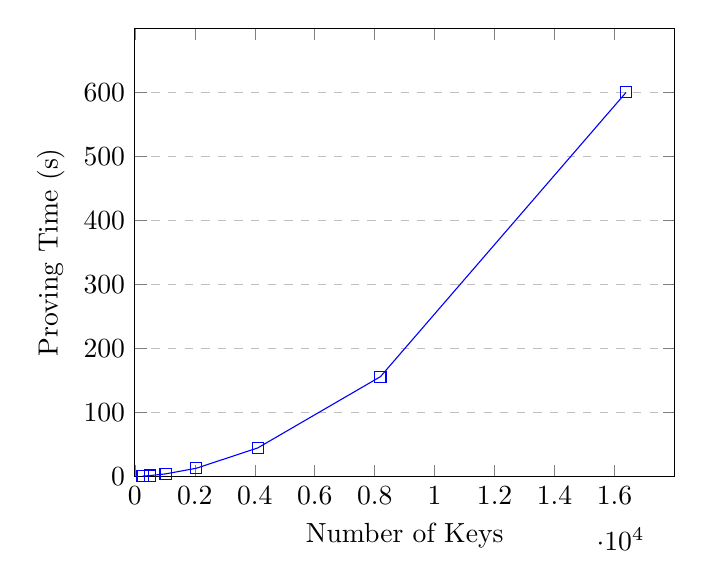
\begin{tikzpicture}
                \begin{axis}[
                    xlabel={Number of Keys},
                    ylabel={Proving Time (s)},
                    xmin=0,xmax=18000,
                    ymin=0,ymax=700,
                    xtick={0,2000,4000,6000,8000,10000,12000,14000,16000},
                    ytick={0,100,200,300,400,500,600},
                    ymajorgrids=true,
                    grid style=dashed,
                ]
                \addplot[
                    color=blue,
                    mark=square,
                ]
                    coordinates {
                        (256,0.63)(512,1.48)(1024,4.11)(2048,12.9)(4096,44.59)(8192,155.94)(16384,599.78)
                    };
                \end{axis}
            \end{tikzpicture}
        }
        \subcaption{}
    \end{subfigure}
    \begin{subfigure}{0.3\textwidth}
        \centering
        \resizebox{\linewidth}{!}{
            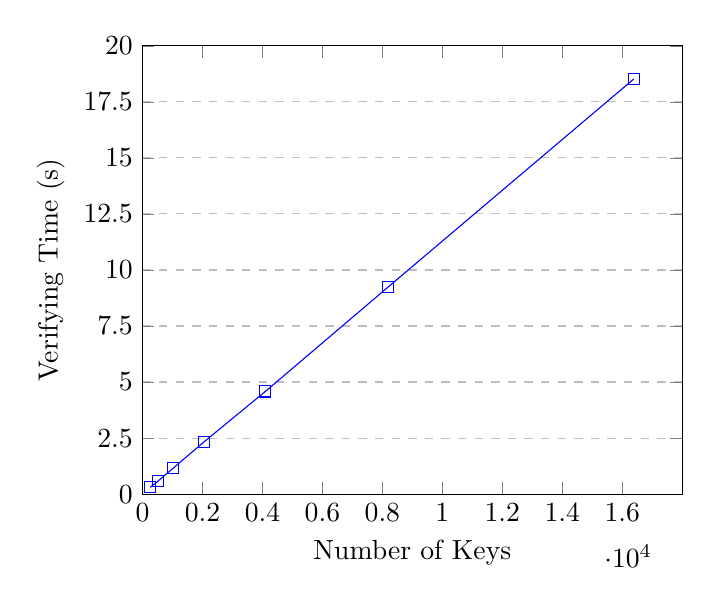
\begin{tikzpicture}
                \begin{axis}[
                    xlabel={Number of Keys},
                    ylabel={Verifying Time (s)},
                    xmin=0,xmax=18000,
                    ymin=0,ymax=20,
                    xtick={0,2000,4000,6000,8000,10000,12000,14000,16000},
                    ytick={0,2.5,5,7.5,10,12.5,15,17.5,20},
                    ymajorgrids=true,
                    grid style=dashed,
                ]
                \addplot[
                    color=blue,
                    mark=square,
                ]
                    coordinates {
                        (256,0.3)(512,0.58)(1024,1.16)(2048,2.33)(4096,4.58)(8192,9.24)(16384,18.52)
                    };
                \end{axis}
            \end{tikzpicture}
        }
        \subcaption{}
    \end{subfigure}
    \begin{subfigure}{0.3\textwidth}
        \centering
        \resizebox{\linewidth}{!}{
            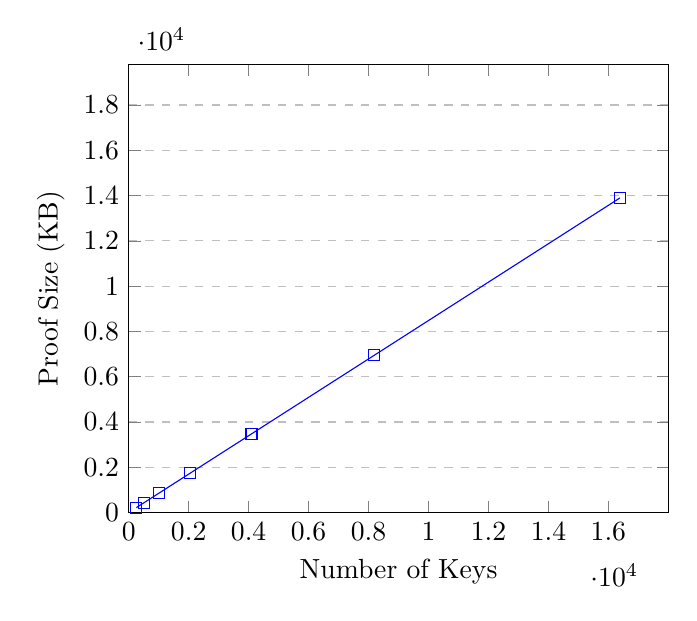
\begin{tikzpicture}
                \begin{axis}[
                    xlabel={Number of Keys},
                    ylabel={Proof Size (KB)},
                    xmin=0,xmax=18000,
                    ymin=0,ymax=19800,
                    xtick={0,2000,4000,6000,8000,10000,12000,14000,16000},
                    ytick={0,2000,4000,6000,8000,10000,12000,14000,16000,18000,20000},
                    ymajorgrids=true,
                    grid style=dashed,
                ]
                \addplot[
                    color=blue,
                    mark=square,
                ]
                    coordinates {
                        (256,217.0)(512,434.0)(1024,868.0)(2048,1736.0)(4096,3473.0)(8192,6946.0)(16384,13893.0)
                    };
                \end{axis}
            \end{tikzpicture}
        }
        \subcaption{}
    \end{subfigure}
\caption{Performance of \bootstrap. Subfigure (a) illustrates the number of keys and the proving time; Subfigure (b) and (c) indicate the verifying time and the proof size are linear in the number of keys.}
\end{figure*}

\begin{figure*}[t]
    \begin{subfigure}{0.3\textwidth}
        \resizebox{\linewidth}{!}{
            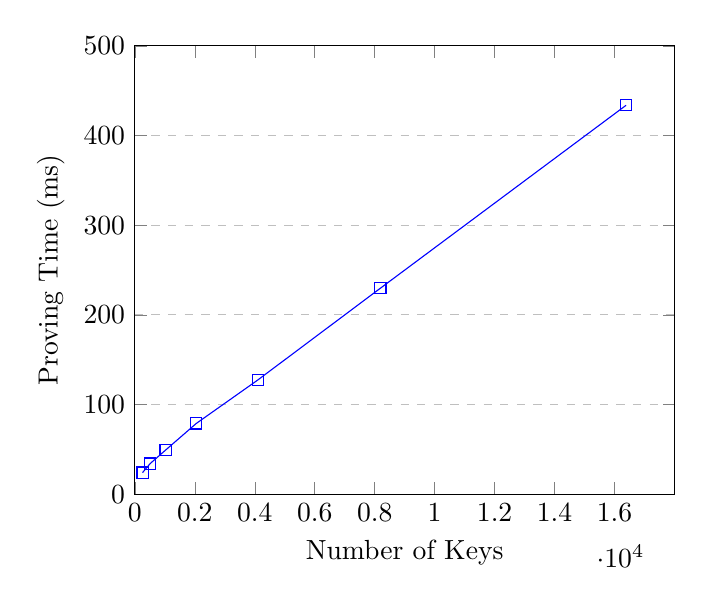
\begin{tikzpicture}
                \begin{axis}[
                    xlabel={Number of Keys},
                    ylabel={Proving Time (ms)},
                    xmin=0,xmax=18000,
                    ymin=0,ymax=500,
                    xtick={0,2000,4000,6000,8000,10000,12000,14000,16000},
                    ytick={0,100,200,300,400,500},
                    ymajorgrids=true,
                    grid style=dashed,
                ]
                \addplot[
                    color=blue,
                    mark=square,
                ]
                    coordinates {
                        (256,24.02)(512,34.1)(1024,49.09)(2048,78.8)(4096,127.17)(8192,229.71)(16384,433.66)
                    };
                \end{axis}
            \end{tikzpicture}
        }
        \subcaption{}
    \end{subfigure}
    \begin{subfigure}{0.3\textwidth}
        \resizebox{\linewidth}{!}{
            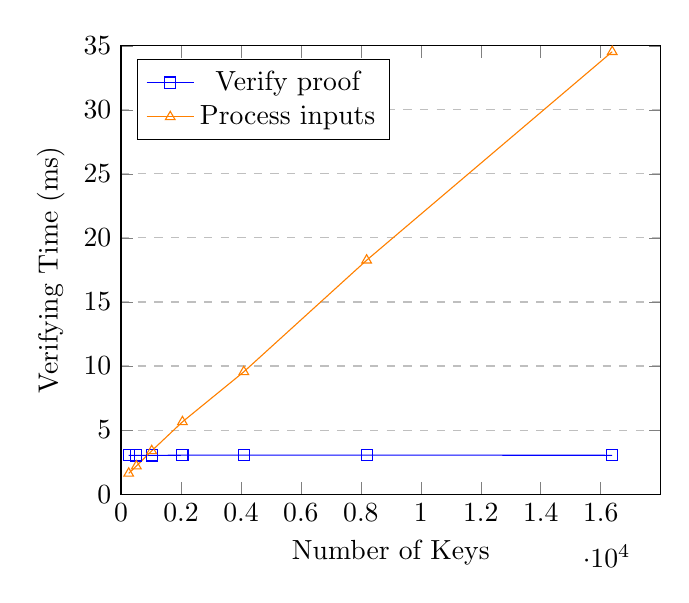
\begin{tikzpicture}
                \begin{axis}[
                    xlabel={Number of Keys},
                    ylabel={Verifying Time (ms)},
                    xmin=0,xmax=18000,
                    ymin=0,ymax=35,
                    xtick={0,2000,4000,6000,8000,10000,12000,14000,16000},
                    ytick={0,5,10,15,20,25,30,35},
                    ymajorgrids=true,
                    grid style=dashed,
                    legend pos=north west,
                ]
                \addplot[
                    color=blue,
                    mark=square,
                ]
                    coordinates {
                        (256,3.03)(512,3.02)(1024,3.02)(2048,3.04)(4096,3.04)(8192,3.05)(16384,3.03)
                    };
                \addlegendentry{Verify proof}

                \addplot[
                    color=orange,
                    mark=triangle,
                ]
                    coordinates {
                        (256,1.62)(512,2.19)(1024,3.38)(2048,5.64)(4096,9.55)(8192,18.26)(16384,34.54)
                    };
                \addlegendentry{Process inputs}
                \end{axis}
            \end{tikzpicture}
        }
        \subcaption{}
    \end{subfigure}
    \begin{subfigure}{0.3\textwidth}
        \resizebox{\linewidth}{!}{
            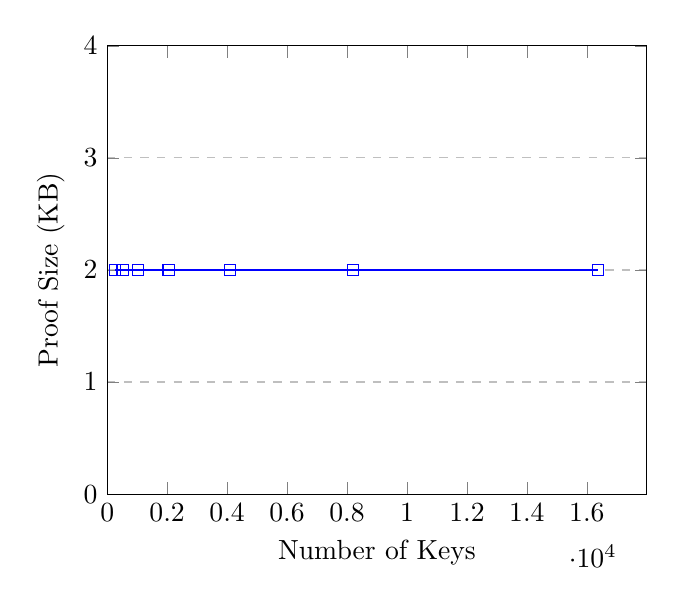
\begin{tikzpicture}
                \begin{axis}[
                    xlabel={Number of Keys},
                    ylabel={Proof Size (KB)},
                    xmin=0,xmax=18000,
                    ymin=0,ymax=4,
                    xtick={0,2000,4000,6000,8000,10000,12000,14000,16000},
                    ytick={0,1,2,3,4},
                    ymajorgrids=true,
                    grid style=dashed,
                ]
                \addplot[
                    color=blue,
                    mark=square,
                ]
                    coordinates {
                        (256,2.0)(512,2.0)(1024,2.0)(2048,2.0)(4096,2.0)(8192,2.0)(16384,2.0)
                    };
                \end{axis}
            \end{tikzpicture}
        }
        \subcaption{}
    \end{subfigure}
\caption{Performance of \poa. Subfigure (a) and (b) suggest the proving time and the verifying time are linear in the number of keys; Subfigure (c) shows the proof size is constant, 2KB, based on our implementation.}
\end{figure*}

\begin{figure*}[t]
    \begin{subfigure}{0.5\textwidth}
        \resizebox{\linewidth}{!}{
            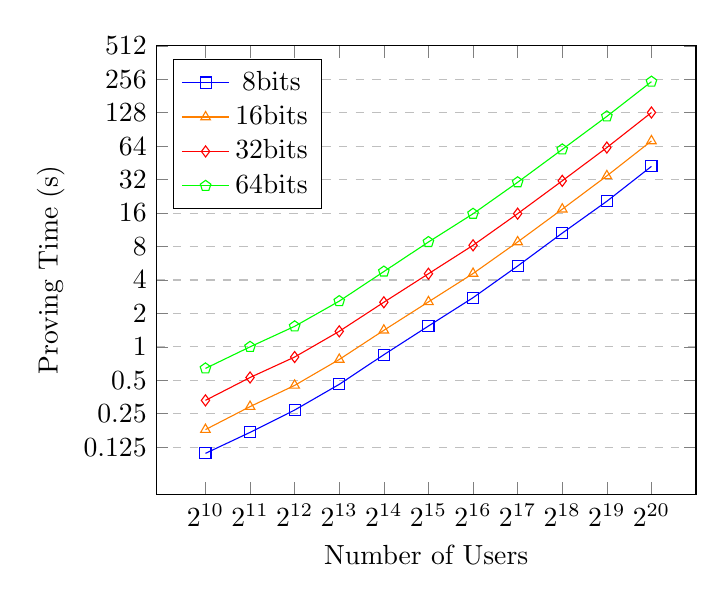
\begin{tikzpicture}
                \begin{loglogaxis}[
                    xlabel={Number of Users},
                    ylabel={Proving Time (s)},
                    xmin=0,xmax=2097152,
                    ymin=0,ymax=512,
                    xtick={0,1024,2048,4096,8192,16384,32768,65536,131072,262144,524288,1048576},
                    ytick={0,0.125,0.25,0.5,1,2,4,8,16,32,64,128,256,512},
                    xticklabels={$2^{10}$,$2^{11}$,$2^{12}$,$2^{13}$,$2^{14}$,$2^{15}$,$2^{16}$,$2^{17}$,$2^{18}$,$2^{19}$,$2^{20}$},
                    yticklabels={0.125,0.25,0.5,1,2,4,8,16,32,64,128,256,512},
                    ymajorgrids=true,
                    grid style=dashed,
                    legend pos=north west,
                ]
                \addplot[
                    color=blue,
                    mark=square,
                ]
                    coordinates {
                        (1024,0.11)(2048,0.17)(4096,0.27)(8192,0.46)(16384,0.85)(32768,1.54)(65536,2.77)(131072,5.34)(262144,10.56)(524288,20.43)(1048576,42.1)
                    };
                \addlegendentry{8bits}

                \addplot[
                    color=orange,
                    mark=triangle,
                ]
                    coordinates {
                        (1024,0.18)(2048,0.29)(4096,0.45)(8192,0.77)(16384,1.41)(32768,2.54)(65536,4.57)(131072,8.79)(262144,17.33)(524288,34.56)(1048576,71.31)
                    };
                \addlegendentry{16bits}

                \addplot[
                    color=red,
                    mark=diamond,
                ]
                    coordinates {
                        (1024,0.33)(2048,0.53)(4096,0.81)(8192,1.38)(16384,2.52)(32768,4.55)(65536,8.2)(131072,15.8)(262144,31.19)(524288,62.16)(1048576,128.49)
                    };
                \addlegendentry{32bits}

                \addplot[
                    color=green,
                    mark=pentagon,
                ]
                    coordinates {
                        (1024,0.64)(2048,1.0)(4096,1.53)(8192,2.58)(16384,4.76)(32768,8.78)(65536,15.76)(131072,30.27)(262144,59.8)(524288,118.57)(1048576,243.53)
                    };
                \addlegendentry{64bits}

                \end{loglogaxis}
            \end{tikzpicture}
        }
        \subcaption{}
    \end{subfigure}
    \begin{subfigure}{0.5\textwidth}
        \resizebox{\linewidth}{!}{
            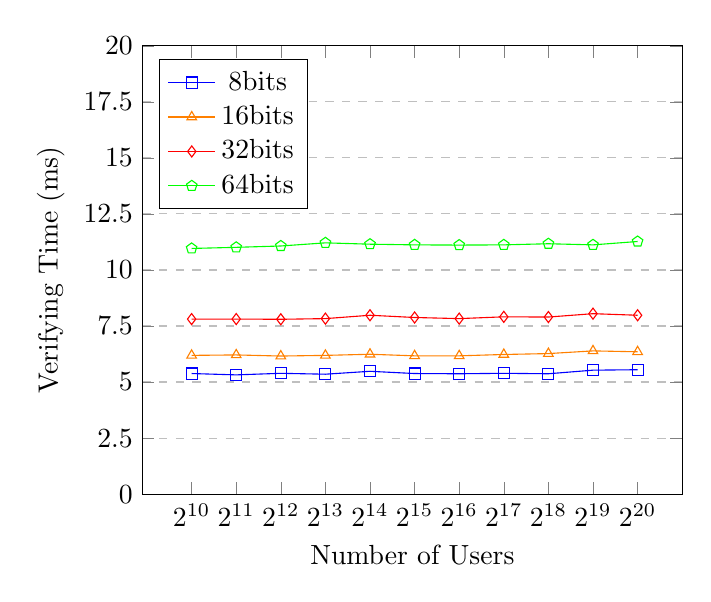
\begin{tikzpicture}
                \begin{semilogxaxis}[
                    xlabel={Number of Users},
                    ylabel={Verifying Time (ms)},
                    xmin=0,xmax=2097152,
                    ymin=0,ymax=20.0,
                    xtick={0,1024,2048,4096,8192,16384,32768,65536,131072,262144,524288,1048576},
                    ytick={0,2.5,5.0,7.5,10.0,12.5,15.0,17.5,20.0},
                    xticklabels={$2^{10}$,$2^{11}$,$2^{12}$,$2^{13}$,$2^{14}$,$2^{15}$,$2^{16}$,$2^{17}$,$2^{18}$,$2^{19}$,$2^{20}$},
                    ymajorgrids=true,
                    grid style=dashed,
                    legend pos=north west,
                ]

                \addplot[
                    color=blue,
                    mark=square,
                ]
                    coordinates {
                        (1024,5.38)(2048,5.32)(4096,5.39)(8192,5.35)(16384,5.48)(32768,5.38)(65536,5.37)(131072,5.39)(262144,5.37)(524288,5.53)(1048576,5.55)
                    };
                \addlegendentry{8bits}

                \addplot[
                    color=orange,
                    mark=triangle,
                ]
                    coordinates {
                        (1024,6.19)(2048,6.21)(4096,6.16)(8192,6.19)(16384,6.24)(32768,6.17)(65536,6.17)(131072,6.23)(262144,6.27)(524288,6.39)(1048576,6.35)
                    };
                \addlegendentry{16bits}

                \addplot[
                    color=red,
                    mark=diamond,
                ]
                    coordinates {
                        (1024,7.81)(2048,7.81)(4096,7.8)(8192,7.83)(16384,7.98)(32768,7.88)(65536,7.83)(131072,7.91)(262144,7.9)(524288,8.05)(1048576,7.98)
                    };
                \addlegendentry{32bits}

                \addplot[
                    color=green,
                    mark=pentagon,
                ]
                    coordinates {
                        (1024,10.96)(2048,11.01)(4096,11.07)(8192,11.21)(16384,11.15)(32768,11.12)(65536,11.11)(131072,11.12)(262144,11.17)(524288,11.12)(1048576,11.27)
                    };
                \addlegendentry{64bits}

                \end{semilogxaxis}
            \end{tikzpicture}
        }
        \subcaption{}
    \end{subfigure}

    \begin{subfigure}{0.5\textwidth}
        \resizebox{\linewidth}{!}{
            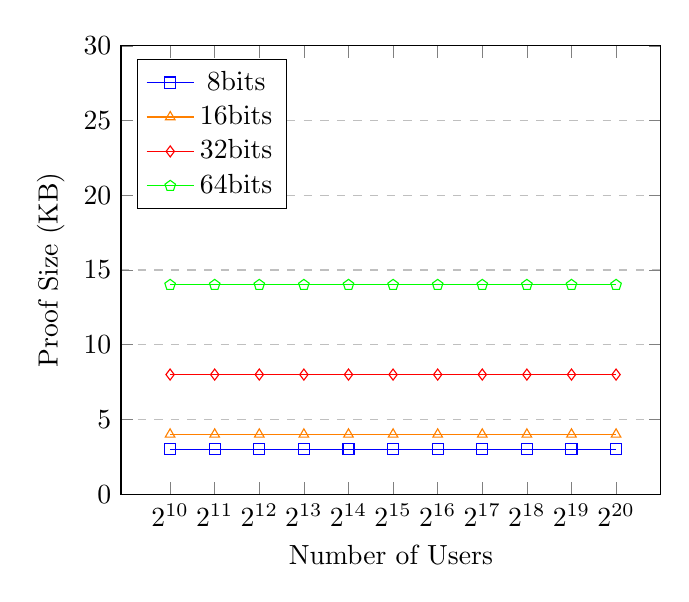
\begin{tikzpicture}
                \begin{semilogxaxis}[
                    xlabel={Number of Users},
                    ylabel={Proof Size (KB)},
                    xmin=0,xmax=2097152,
                    ymin=0,ymax=30,
                    xtick={0,1024,2048,4096,8192,16384,32768,65536,131072,262144,524288,1048576},
                    ytick={0,5,10,15,20,25,30},
                    xticklabels={$2^{10}$,$2^{11}$,$2^{12}$,$2^{13}$,$2^{14}$,$2^{15}$,$2^{16}$,$2^{17}$,$2^{18}$,$2^{19}$,$2^{20}$},
                    ymajorgrids=true,
                    grid style=dashed,
                    legend pos=north west,
                ]

                \addplot[
                    color=blue,
                    mark=square,
                ]
                    coordinates {
                        (1024,3.0)(2048,3.0)(4096,3.0)(8192,3.0)(16384,3.0)(32768,3.0)(65536,3.0)(131072,3.0)(262144,3.0)(524288,3.0)(1048576,3.0)
                    };
                \addlegendentry{8bits}

                \addplot[
                    color=orange,
                    mark=triangle,
                ]
                    coordinates {
                        (1024,4.0)(2048,4.0)(4096,4.0)(8192,4.0)(16384,4.0)(32768,4.0)(65536,4.0)(131072,4.0)(262144,4.0)(524288,4.0)(1048576,4.0)
                    };
                \addlegendentry{16bits}

                \addplot[
                    color=red,
                    mark=diamond,
                ]
                    coordinates {
                        (1024,8.0)(2048,8.0)(4096,8.0)(8192,8.0)(16384,8.0)(32768,8.0)(65536,8.0)(131072,8.0)(262144,8.0)(524288,8.0)(1048576,8.0)
                    };
                \addlegendentry{32bits}

                \addplot[
                    color=green,
                    mark=pentagon,
                ]
                    coordinates {
                        (1024,14.0)(2048,14.0)(4096,14.0)(8192,14.0)(16384,14.0)(32768,14.0)(65536,14.0)(131072,14.0)(262144,14.0)(524288,14.0)(1048576,14.0)
                    };
                \addlegendentry{64bits}

                \end{semilogxaxis}
            \end{tikzpicture}
        }
        \subcaption{}
    \end{subfigure}
\caption{Performance of PoL by different number of bits for the range proof. Subfigure (a) illustrates the proving time linearly relates to the number of users, and it is also linear to the number of bits for the same number of users; Subfigure (b) and (c) show the verifying time and the proof size are unrelated to the number of users, but relate to the number of bits. Unlike the proving time, the verifying time and the proof size do not linearly increase following the number of bits.\label{fig:pol}}
\end{figure*}


To evaluate the performance of \Sys, we implemented our protocols in Rust based on the popular library, arkworks\footnote{\url{https://github.com/arkworks-rs}}. Our implementation is publicly accessible on GitHub\footnote{GitHub: link removed for anonymity. Can supply code via the program chairs as necessary.}. We chose the pairing-friendly elliptic curve \bls for the KZG commitment which has 128 bit security.

Our experiments were conducted on a personal computer with i9-13900KF and 32GB of memory. The experimental data including balances and \secp key pairs are randomly generated locally for simplicity. Since there is no range-proof for PoA, we tested the PoA with balances randomly distributed in $[1,2^{64})$ to simulate the real distribution of assets, and for PoL, we tested the program with balances randomly distributed in $[1,2^8)$, $[1,2^{16})$, $[1,2^{32})$, and $[1,2^{64})$. We simulated $2^8,2^9\dots,2^{14}$ and $2^{10},2^{11},\dots,2^{20}$ users for PoA and PoL respectively. Simulating different number of users for PoA and PoL is because \bootstrap was time-consuming for larger number of users. For each protocol, we ran the test for ten times with the same experimental data. Our figures are interpolated from the average performance of ten times with discarding the maximum and minimum of the samples.

\section{Experimental Evaluation}
Figure 2, 3, and 4 reflect the performance of \Sys in single thread with i9-13900KF. The Subfigure (a) of Figure 2 suggests it takes around 600 seconds to generate the proofs for 16,384 keys with i9-13900KF for \bootstrap, and the proof size is 13,893KB. There are around $2^{28}$ unique Ethereum addresses reported by Ethercan.io in May 2024 \footnote{\url{https://etherscan.io/chart/address}}, which means it requires 9,830,400 computing instances to generate the proofs for all the keys in 600 seconds if the exchange wants the maximum anonymous set. It seems impractical for the exchange to deploy such number of servers in the real world. However, recall the exchange only needs to perform \bootstrap once. The exchange can sacrifice the proving time to reduce the number of servers. Moreover, the proving time can be reduced significantly if manipulating more efficient KZG opening schemes. See Section~\ref{sec:opt} for more detailed optimizations. 

Figure 3 shows the proving time and the verifying time are linear in the number of the keys. In our experiments, it takes 433.66 milliseconds to generate the proof and 37.57 milliseconds to verify the proof for 16,384 keys. This suggests the proving time is less than 2 hours if the anonymous set is the whole addresses on Ethereum without any other optimizations! Since the proof size of a KZG commitment is unrelated to the degree of the polynomial (the number of keys), the proof size of \poa is constant (2KB) based on our implementation.

Figure 4 illustrates the performance of our PoL with different number of users and allowed ranges for balance. Our experiments show the proving time grows linearly by the number of users while the verifying time and the proof size are constant. From the test result of Binance's PoL, it needs 1.5 days to generate the proof for 100 million accounts with 100 servers \footnote{\url{https://github.com/binance/zkmerkle-proof-of-solvency/?tab=readme-ov-file}}, but our PoL requires less than 10 minutes with the same number of servers. This indicates our protocol is practical to handle the real-world applications.

\section{Optimization}
\label{sec:opt}
Due to the additively homomorphic property of KZG commitment, the prover's work in our protocols can be easily assigned into arbitrary number of servers, and there is no need to provide extra proofs to aggregate the proofs from different servers (provers). That means the proving time will decrease with the growing number of servers. This is the most direct method to make the protocols more efficient. Another way to improve the performance without adding more servers is utilizing more efficient KZG opening schemes. Recall the heaviest work of \bootstrap is proving each committed point is correct, and the opening scheme we demonstrated from Plonk requires $t\cdot{d}$ scalar multiplications for prover, where $t$ is the number of the opening points and $d$ is the degree bound of the polynomial. The work in BDFG20~\cite{bdfg} can reduce this complexity to $2n$ scalar multiplications, which means the dominating complexity will become $O(n)$ rather than $O(n^2)$. The aggregation slightly increases the verifier's work but the extra cost is trivial because of the succinctness of KZG commitment scheme. These optimizations can be applied to both of our PoA and PoL. Moreover, the proof length for multiple points of the KZG commitment will also be decreased to $O(1)$ if BDFG20 is integrated, but the total proof length is still $O(n)$ because of the proof of the $\Sigma$-protocol.

% = = = = = = = = = = = = = = = = = = = = = = = = = = = = = = = = = = =